\documentclass{beamer}
\mode<presentation> {
\usetheme{tcd}
\usepackage{url}
\usepackage{listings}
\usepackage{color}
\usepackage{verbatim}
\usepackage{graphicx}
\usepackage{ulem}

\definecolor{dkgreen}{rgb}{0,0.6,0}
\definecolor{gray}{rgb}{0.5,0.5,0.5}
\definecolor{mauve}{rgb}{0.58,0,0.82}

%\lstset{frame=tb,
%  language=C,
%  aboveskip=3mm,
%  belowskip=3mm,
%  showstringspaces=false,
%  columns=flexible,
%  basicstyle={\small\ttfamily},
%  numbers=none,
%  numberstyle=\tiny\color{gray},
%  keywordstyle=\color{blue},
%  commentstyle=\color{dkgreen},
%  stringstyle=\color{mauve},
%  breaklines=true,
%  breakatwhitespace=true,
%  tabsize=3
%}
}

\title[]{ALT SRE}

\author{Sean McGrath}
\institute[TCD]
{
Resarch IT \\
Trinity College Dublin \\
\medskip
\textit{sean.mcgrath@tcd.ie} 
}
\date{8th November 2018}

\begin{document}

\begin{frame}
\titlepage
\end{frame}

\begin{frame}
\frametitle{SRE – Site/System Reliability Engineering}

Typical SRE activities fall into some of the following categories
\footnote{\url{https://landing.google.com/sre/book/chapters/eliminating-toil.html}}

\begin{itemize}
\item Software engineering
	\begin{itemize}
	\item E.g. automation scripts, ... adding service features for scalability and reliability, or modifying infrastructure to make it more robust.
	\end{itemize}
\item Systems engineering
	\begin{itemize}
	\item E.g. Configuring production systems, modifying configurations. 
	\end{itemize}
\item Toil
	\begin{itemize}
	\item the kind of work tied to running a production service that tends to be manual, repetitive, automatable, tactical, devoid of enduring value, and that scales linearly as a service grows.
	\end{itemize}
\end{itemize}
\begin{quote}
"Simply put, SRE is software engineering applied to operations"
\footnote{\url{https://www.lynda.com/Software-Development-tutorials/DevOps-Foundations-Site-Reliability-Engineering/669542-2.html}}
\end{quote}
\end{frame}

\begin{frame}
\frametitle{What does "ALT" mean?}
	\begin{itemize}
	\item Short for alternative
	\item Alternative Site Reliability Engineering, (ALT SRE), is like the SRE Google does, but not as good
	\item It's much worse actually!
	\end{itemize}
    \begin{center}
     
\includegraphics[width=0.5\textwidth]{imgs/kellyanne.png}
     \end{center}
\end{frame}

\begin{frame}
\begin{center}
	
\includegraphics[width=0.5\textwidth]{imgs/picard.jpg}
\end{center}
\end{frame}

\begin{frame}
\begin{center}
	
\includegraphics[width=0.5\textwidth]{imgs/scienceguy.jpg}
\end{center}
\end{frame}

\begin{frame}
\frametitle{What's a HPC Cluster?}
Cluster's have lots of nodes that can sometimes fail for varying reasons, (often because the end user does cunning things to break them).
    \begin{center}
     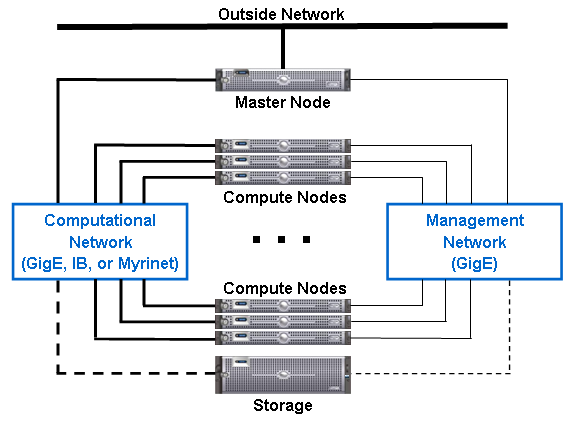
\includegraphics[width=0.5\textwidth]{imgs/cluster_anatomy.png}
     \end{center}
\end{frame}

\begin{frame}
\frametitle{Cluster's in Trinity}
\begin{center}
	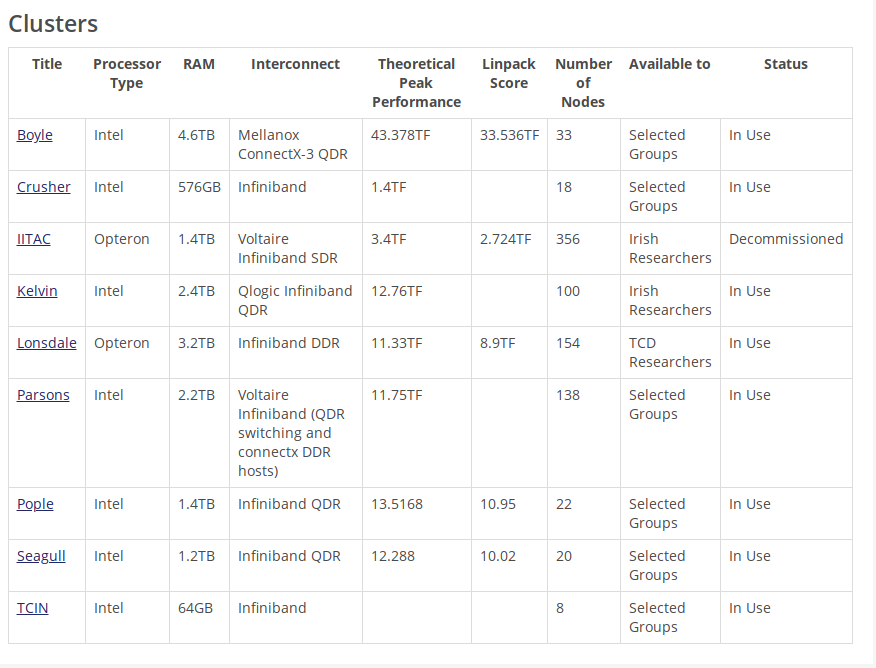
\includegraphics[width=0.75\textwidth]{imgs/tchpc_clusters.png}
\end{center}
\end{frame}

\begin{frame}
\frametitle{Cluster's in Trinity}
\begin{center}
	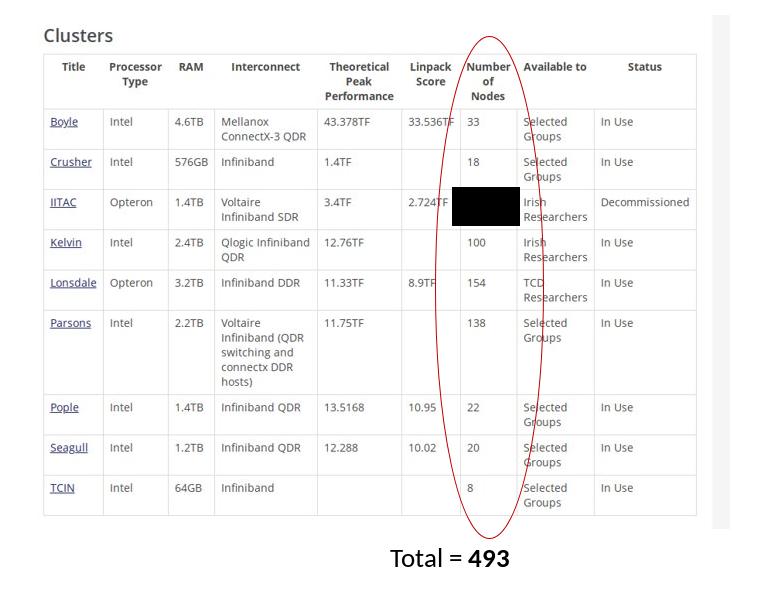
\includegraphics[width=0.75\textwidth]{imgs/tchpc_clusters2.png}
\end{center}
\end{frame}

\begin{frame}
\frametitle{That seems like a lot of servers that could break from time to time}
\begin{center}
	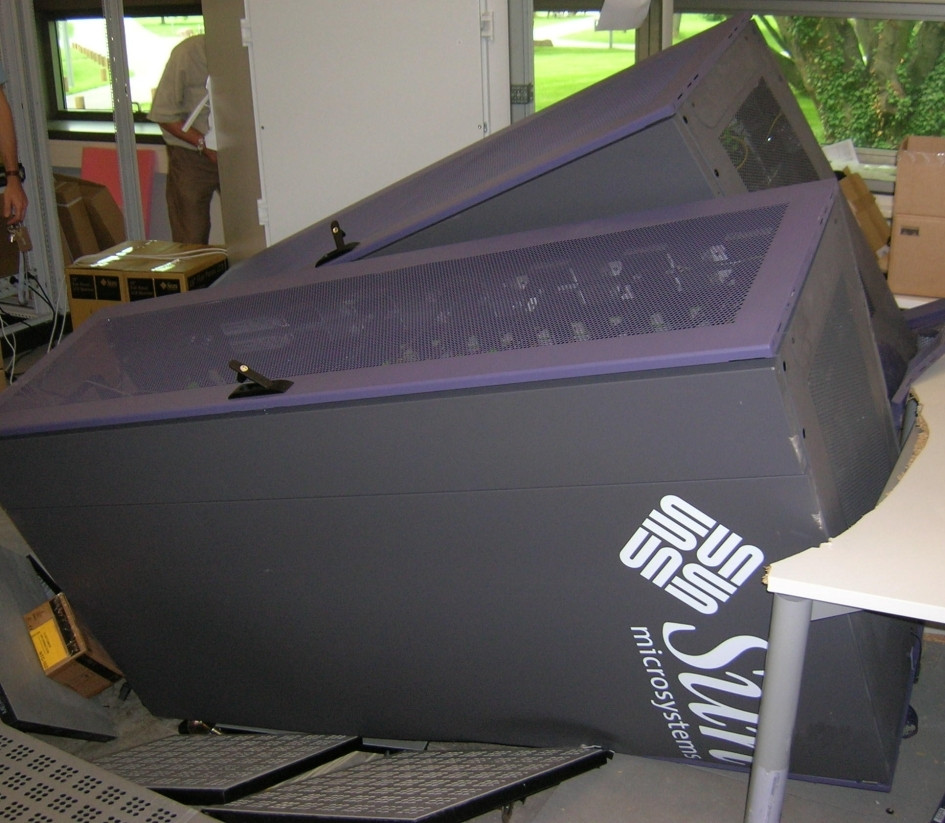
\includegraphics[width=0.75\textwidth]{imgs/fallen_rack.jpg}
\end{center}
\end{frame}

\begin{frame}
\frametitle{What my mornings used to look like}
\begin{enumerate}
	\item Check for whats broken
	\item Perform an action from a small list of common actions on the nodes based on what the queue management software tells you. E.g.
	\begin{enumerate}
		\item Reboot the node to clear out of memory errors
		\item Restart certain services
		\item Etc.
	\end{enumerate}
\end{enumerate}
Repeat until all the nodes are back healthy or I get distracted.\\~\\
A lot of work that was
\begin{itemize}
	\item Manual
	\item Repetitive
	\item Automatable
	\item Tactical
	\item Scaled linearly as a service grow
\end{itemize}
I.E. Toil
\end{frame}

\begin{frame}
\frametitle{Remind you of anything}
    \begin{center}
     
\includegraphics[width=0.5\textwidth]{imgs/bird.jpg}
     \end{center}
\end{frame}

\begin{frame}
\frametitle{The solution?}
    \begin{center}
     
\includegraphics[width=0.5\textwidth]{imgs/automate.jpeg}
     \end{center}
\end{frame}

\begin{frame}
\frametitle{What does ALT SRE look like in TCD?}
\begin{itemize}
	\item An in house developed automation tool, (I.e. a script),
	\item That ties together the common tools, (sometimes just as simple as 'service blah restart' on a server, or remotely power cycling it), 
	\item Run periodically to get the clusters to heal themselves of common problems and free up staff for other, higher order, tasks.
	\item https://github.com/smcgrat/linux-general/blob/master/self-heal.sh
\end{itemize}
\end{frame}

\begin{frame}[fragile]
\frametitle{Examples of what is looked for}
\begin{verbatim}
declare -a nodes_with_problems
declare -a nodes_down_with_HC_errors
declare -a nodes_that_need_cluster_tests_run
declare -a nodes_that_are_draining
declare -a nodes_not_responding
declare -a nodes_with_epilog_errors
\end{verbatim}
\end{frame}

\begin{frame}[fragile]
\frametitle{Example of what it might do}
\begin{lstlisting}[basicstyle=\tiny,]
function restartnode {
        local node=$1
        if [ "$dryrunmode" != "on" ]; then
                if [ "$quorumnode" == "no" ]; then # this is not a member of the quorum, safe to reboot
                        /usr/bin/scontrol reboot_nodes $node
                        echo "$node rebooting"
                        operation="$operation node rebooted - "
                else 
                        echo "$node is a quorum node - don't reboot"
                        supdate $node drain "SH:OOMquorumnode"
                        operation="$operation quorum node that needs a reboot - "
                fi
        else
                echo "$node - services not being restarted as script has been run in dry run mode"
                operation="$operation node rebooted - "
        fi
}
\end{lstlisting}
\end{frame}

\begin{frame}
\frametitle{Comments / Observations}
Some of the poor design decisions made along the way
\begin{itemize}
	\item Writing it in bash!
	\item Particularly not a 686 line bash script. That’s just silly
\end{itemize}
Some of the pitfalls of having a self healing cluster
\begin{itemize}
	\item Sometimes you actually want your cluster to be off, so having a tool that automatically turns it back on may not be optimal!
\end{itemize}
Some possible future developments
\begin{itemize}
	\item Re-write in Python
	\item Write as a state machine
\end{itemize}
\end{frame}

\begin{frame}
\frametitle{Thank You!}
\begin{center}
	Questions?
\end{center}
\end{frame}
\end{document}
